\section{Theoretical Analysis}
\label{sec:analysis}

We analyse the circuit shown in Figure~\ref{fig:rc} for t<0 using the nodal method.
The nodes are numbered according to what's shown in the picture.
In this first instance we are working in a steady state, where no current is flowing through the capacitor: we can replace it with an open circuit.
After doing this, it is clear that all the components we are working with are linear and so we will need to solve a system of linear equations to determine the initial values for the subsequent analysis.
This way, we’ve ran the nodal method and solved the linear system on GNU Octave.
\subsection{Node Analysis for t<0}
Knowing that V4=0 since it is connected to the ground:
\begin{equation}
\begin{pmatrix}
1 & 0 & 0 & 0 & 0 & 0 & 0\\
-G1 & G1+G2+G3 & -G2 & -G3 & 0 & 0 & 0\\
0 & Kb+G2 & -G2 & -Kb & 0 & 0 & 0\\
-G1 & G1 & 0 & G4 & 0 & G6 & 0\\
0 & 0 & 0 & 0 & 0 & -G6-G7 & G7\\
0 & 0 & 0 & 1 & 0 & G6*Kd & -1\\
0 & -G3 & 0 & G3+G4+G5 & -G5 & G6 & 0
\end{pmatrix}
\begin{pmatrix}
V1\\
V2\\
V3\\
V5\\
V6\\
V7\\
V8
\end{pmatrix}
=
\begin{pmatrix}
Vs\\
0\\
0\\
0\\
0\\
0\\
0
\end{pmatrix}
\end{equation}
We can also easily obtain the current values in the various branches through Ohm's law. This yields the following results:
\begin{table}[h]
  \centering
  \begin{tabular}{|l|r|}
    \hline    
    {\bf Name} & {\bf Value [A and V]} \\ \hline
    @gb[i] & -2.29771e-04\\ \hline
@idd[current] & 1.005042e-03\\ \hline
@r1[i] & 2.191669e-04\\ \hline
@r2[i] & 2.297712e-04\\ \hline
@r3[i] & 1.060424e-05\\ \hline
@r4[i] & 1.185502e-03\\ \hline
@r5[i] & 1.234813e-03\\ \hline
@r6[i] & 9.663347e-04\\ \hline
@r7[i] & 9.663347e-04\\ \hline
v(1) & -9.73914e-01\\ \hline
v(3) & 1.063433e+01\\ \hline
v(4) & 6.382611e+00\\ \hline
v(5) & 6.843347e+00\\ \hline
v(6) & 7.067298e+00\\ \hline
v(7) & 1.953900e+00\\ \hline
v(8) & 6.875344e+00\\ \hline
v(9) & 0.000000e+00\\ \hline
 
  \end{tabular}
  \caption{Theoretical analysis results. (A variable preceded by @ is of type {\em current})}
  \label{tab:nodal}
\end{table}

\subsection{Equivalent Resistor}
In order to compute the equivalent resistor we ran a nodal analysis, making Vs=0 and replacing the capacitor with a voltage source Vx=V6-V8 as calculated in the previous step. This is made to ensure that the voltage in the capacitor is continuous since it does so in reality: this is a capacitor discharging through a resistance, any discontinuity in voltage would require an infinite amount of current. 
\begin{equation}
\begin{pmatrix}
1 & 0 & 0 & 0 & 0 & 0 & 0\\
-G1 & G1+G2+G3 & -G2 & -G3 & 0 & 0 & 0\\
0 & Kb+G2 & -G2 & -Kb & 0 & 0 & 0\\
-G1 & G1 & 0 & G4 & 0 & G6 & 0\\
0 & 0 & 0 & 0 & 0 & -G6-G7 & G7\\
0 & 0 & 0 & 1 & 0 & G6*Kd & -1\\
0 & 0 & 0 & 0 & 1 & 0 & -1
\end{pmatrix}
\begin{pmatrix}
V1\\
V2\\
V3\\
V5\\
V6\\
V7\\
V8
\end{pmatrix}
=
\begin{pmatrix}
0\\
0\\
0\\
0\\
0\\
0\\
Vx
\end{pmatrix}
\end{equation}

With the following definitions:
\begin{equation}
V_x=V_6-V_8;
\end{equation}
\begin{equation}
I_x=\frac {V_6-V_5}{R_5}+\frac {V_3-V_2}{R_2};
\end{equation}
\begin{equation}
Req=\frac {V_x}{I_x}
\end{equation}
We were able to obtain the following values, laying the foundation for the natural solution:
\begin{table}[h]
  \centering
  \begin{tabular}{|l|r|}
    \hline    
    {\bf Name} & {\bf Value} \\ \hline
    $V_{x}$ & 8.548721 V\\ \hline
@$I_{x}$ & 2.808224 mA\\ \hline
$R_{eq}$ & 3.044174 kOhm\\ \hline
$tau$ & 3.059522 ms\\ \hline 
  \end{tabular}
  \caption{Nodal analysis results.}
  \label{tab:nodal}
\end{table}
\subsection{Natural solution}
The general solution for RC circuits, making use of the computations in the previous section, yields:
\begin{equation}
V_{6n}(t)=V_xexp(-\frac{t}{RC})
\end{equation}
From this equation, we obtained the following plot, which depicts the first twenty milisseconds of the circuit's natural response.
\begin{figure}[h] \centering
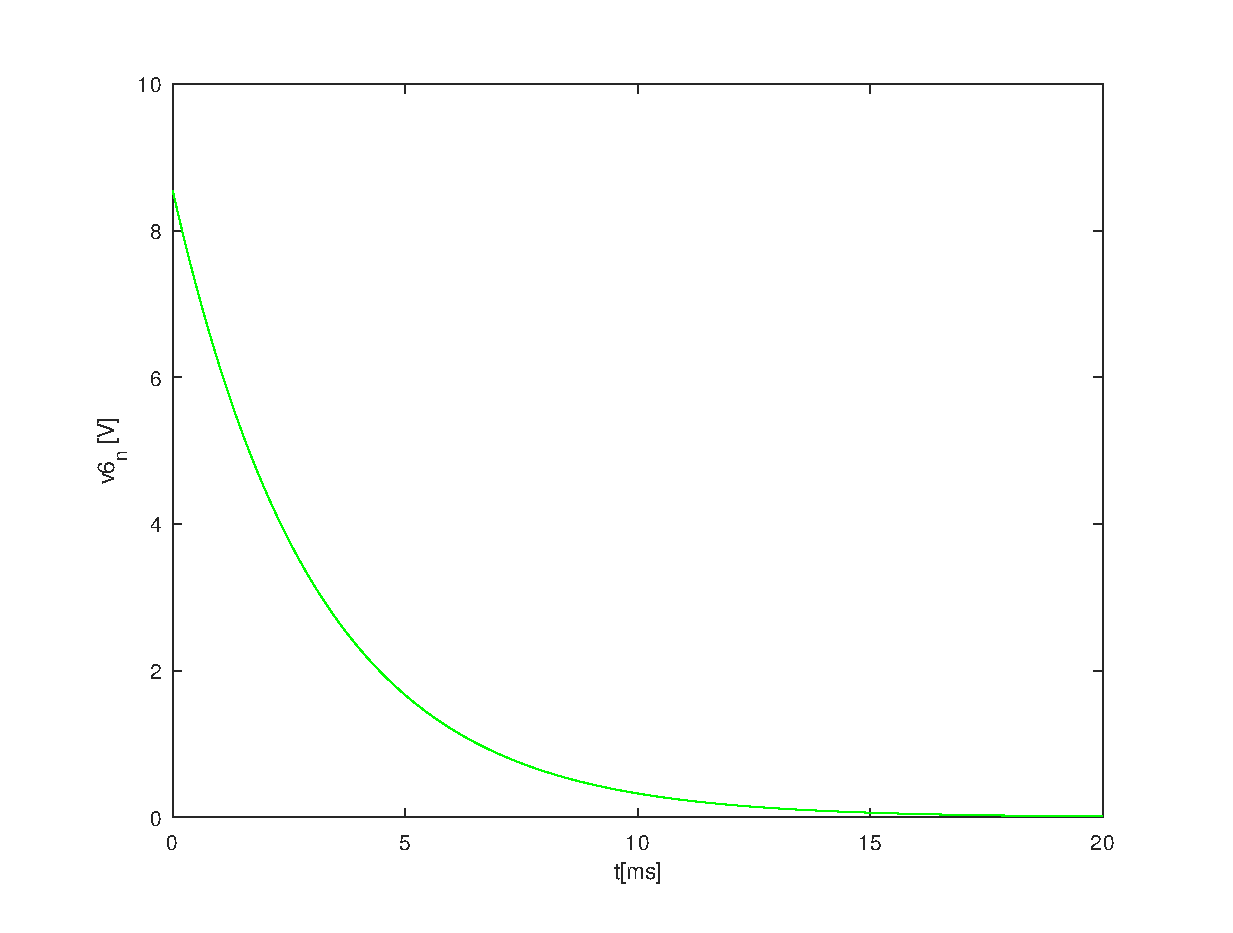
\includegraphics[width=0.8\linewidth]{natural.eps}
\caption{Natural solution to $V_{6}$ node voltage.}
\label{fig:current}
\end{figure}

\subsection{Forced and final total solution}

\begin{figure}[h] \centering
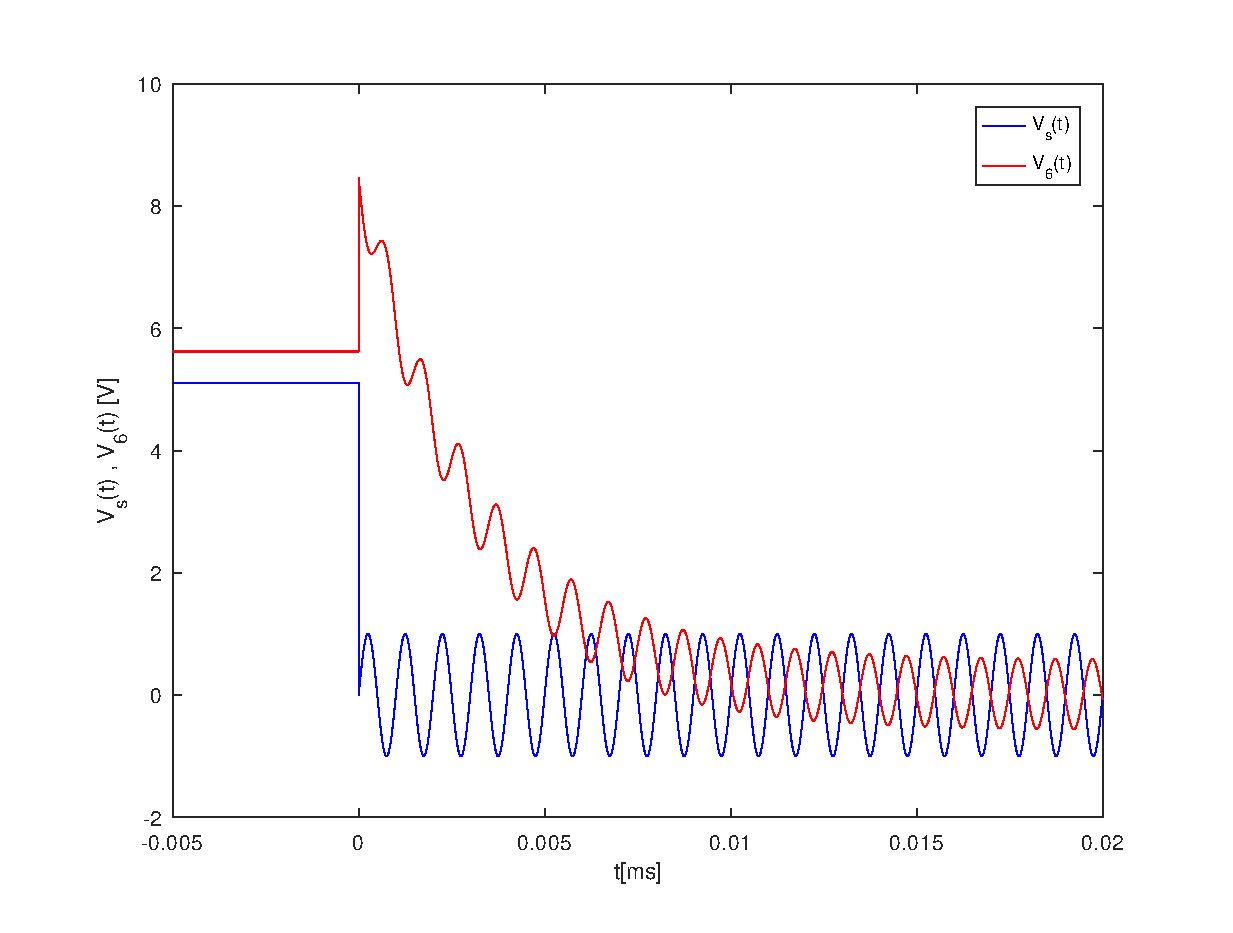
\includegraphics[width=0.8\linewidth]{total.eps}
\caption{Total solution to $V_{6}$ node voltage.}
\label{fig:current}
\end{figure}

\subsection{Node Analysis}

As in the previous section, we extract a set of equations from the circuit, this time using the node method. This yields 8 equations, one for each node. Then, we can solve those 8 equations in the form of the matrix presented here.
\begin{equation}
\begin{pmatrix}
G7 & 0 & 0 & 0 & 0 & 0 & G6 & 0\\
1 & -1 & 0 & 0 & 0 & 0 & 0 & 0\\
0 & 0 & 0 & 0 & 0 & 1 & -1 & 0\\
0 & 0 & 0 & -G2 & G1+G2+G3 & -G1 & 0 & -G3\\
0 & 0 & G5 & 0 & G3 & 0 & G4+G6 & -G3-G4-G5\\
1 & 0 & 0 & 0 & 0 & 0& Kc*G6 & -1\\
0 & 0 & 0 & 0 & G1 & -G1 & -G4-G6 & G4\\
0 & 0 & 0 & -G2 & Kb+G2 & 0 & 0 & -Kb
\end{pmatrix}
\begin{pmatrix}
V1\\
V2\\
V3\\
V4\\
V5\\
V6\\
V7\\
V8
\end{pmatrix}
=
\begin{pmatrix}
0\\
0\\
V\\
0\\
I\\
0\\
0\\
0
\end{pmatrix}
\end{equation}

